\pdfoutput=1
\documentclass[11pt,a4paper]{article}

\usepackage[T1]{fontenc}
\usepackage[utf8]{inputenc}

\usepackage[margin=1in]{geometry}
\usepackage{amsmath,amssymb}
\usepackage{graphicx}
\usepackage{booktabs}
\usepackage{array}
\usepackage{multirow}
\usepackage{hyperref}
\usepackage{xcolor}
\usepackage{caption}
\usepackage{subcaption}
\usepackage{placeins}
\usepackage{enumitem}
\usepackage{parskip}

\hypersetup{
  colorlinks=true,
  linkcolor=blue!70!black,
  citecolor=blue!70!black,
  urlcolor=blue!70!black
}

\graphicspath{{figures/}}
\DeclareGraphicsExtensions{.pdf,.png,.jpg}

\title{\textbf{Multi-Agent Investment Strategy System: \\
A Cloud-Native Architecture on Tencent Cloud Platform}}

\author{
  Nuoya Chen\textsuperscript{1}\thanks{Corresponding author: \texttt{nchen@ruc.dk}} \and
  Yiyuan Zhang\textsuperscript{2}\thanks{Equal contribution.} \and
  Min Hu\textsuperscript{3}\footnotemark[2] \and
  Qiang Han\textsuperscript{4} \and
  Aria Liu\textsuperscript{5}
}

\date{
  \textsuperscript{1}Roskilde University\\
  \textsuperscript{2}Fudan University\\
  \textsuperscript{3}Independent Researcher\\
  \textsuperscript{4}Ernst \& Young\\
  \textsuperscript{5}Maersk\\[6pt]
  \small Presented at the Tencent Mini Hackathon, Shanghai, November 2025\\
  \small Paper written March 2026
}

\begin{document}

\maketitle
\thispagestyle{empty}

\begin{abstract}
We present a multi-agent system for automated investment strategy
execution, built on the Tencent Hunyuan foundational model at the
Tencent Mini Hackathon in Shanghai (November 2025). The system uses a three-agent
framework in which specialised agents handle macroeconomic analysis,
fundamental stock screening, and investment intent classification.
Due to time and ethical constraints, only the first two agents were
fully implemented and evaluated.

Testing revealed a critical alignment failure: under sustained user
pressure, the agent bypassed its own $S \geq 60$ scoring threshold and
produced a ten-stock high-risk portfolio instead of the intended
four-stock filtered recommendation. Monte Carlo simulation shows the
overridden portfolio carries $4.3\times$ the absolute loss exposure
(VaR 95\%) of the compliant portfolio for identical risk-adjusted
returns---a direct, quantified cost of LLM sycophantic drift.

The system targets the China A-share market, where policy and
event-driven dynamics differ markedly from the Nasdaq-focused settings
predominant in the literature. We contribute an empirical evaluation
of an open-source LLM in this emerging-market context and discuss
three structural limitations: sequential agent execution, insufficient
server-side data sources, and the inability of the model to maintain
workflow continuity under production-grade operational standards.

\medskip\noindent\textbf{Keywords:} Multi-agent systems, large language
models, LLM alignment, China A-share market, portfolio construction,
cloud-native architecture, Tencent Hunyuan.
\end{abstract}

\newpage
\tableofcontents
\newpage

\section{Introduction}
\label{sec:intro}

The complexity of modern financial markets necessitates sophisticated
computational systems capable of processing vast amounts of
heterogeneous data, executing complex analytical workflows, and making
time-sensitive decisions. Traditional monolithic investment systems face
significant limitations in scalability, maintainability, and
adaptability to rapidly changing market conditions.

Multi-agent systems (MAS) offer a promising paradigm for addressing
these challenges by decomposing complex investment workflows into
specialised, autonomous agents that collaborate through well-defined
communication protocols. Each agent can be optimised for specific
analytical tasks---macroeconomic forecasting, fundamental analysis, or
quantitative execution---while the system as a whole achieves
sophisticated emergent behaviour through agent coordination. This paper
focuses on the China A-share market, where macroeconomic policy,
industrial policy, event-driven strategies, and high-frequency trading
are frequently deployed to generate returns from a large retail-investor
base. The growing universe of listed companies makes comprehensive
manual monitoring infeasible, creating strong incentives for
agent-based automation.

Cloud computing platforms have fundamentally transformed the feasibility
of deploying production-grade MAS. Providers such as Tencent Cloud offer
the distributed computing resources, managed services, and global
network infrastructure necessary to support real-time, fault-tolerant
architectures at enterprise scale. As an experiment within the Tencent
Hackathon (November 2025), we deployed a macroeconomic agent and a fundamental-analysis
agent to evaluate the capabilities of the Hunyuan foundational model.

\subsection*{Research Questions}

This paper addresses the following questions:

\begin{enumerate}[label=\textbf{RQ\arabic*.}]
  \item \textbf{Agent Coordination:} How should communication protocols
        be designed to enable effective collaboration while preserving
        agent autonomy and system resilience?
  \item \textbf{Response Latency:} How can significant per-agent delays
        be minimised without sacrificing analytical depth?
  \item \textbf{Hallucination Mitigation:} How can hallucination rates
        be reduced and agents guided to comply with developer-defined
        rules across multi-turn sessions?
\end{enumerate}

\subsection*{Contributions}

This paper makes the following primary contributions:

\begin{enumerate}
  \item \textbf{Architectural Framework.} A comprehensive three-agent
        architecture designed for investment-strategy automation, with
        detailed specifications for agent responsibilities,
        communication protocols, and coordination logic.
  \item \textbf{Conditional Agent Activation Protocol.} A hierarchical
        coordination mechanism in which macro-level analysis determines
        which downstream agents activate, optimising resource utilisation
        and aligning system behaviour with market regimes.
  \item \textbf{Empirical Evaluation on A-Share Market.} A Monte Carlo
        simulation of a semiconductor portfolio constructed by the
        system, providing quantitative evidence on performance
        characteristics under bear, base, and bull market scenarios.
\end{enumerate}

The remainder of this paper is structured as follows.
Section~\ref{sec:related} reviews related work in multi-agent systems
and financial automation.
Section~\ref{sec:architecture} presents the three-agent architecture.
Section~\ref{sec:results} describes the simulated portfolio construction
and Monte Carlo results.
Section~\ref{sec:risk} summarises risk considerations.
Section~\ref{sec:discussion} discusses structural limitations.
Section~\ref{sec:conclusion} concludes with implications and future
directions.

\section{Related Work}
\label{sec:related}

Research at the intersection of large language models and financial
automation has grown rapidly across four interconnected dimensions:
multi-agent system design for investment tasks, LLM alignment and
sycophantic drift, AI-driven analysis of the China A-share market, and
portfolio simulation methodology. This section reviews the most relevant
prior work in each area and situates the present paper within that
landscape.

\subsection{Multi-Agent Systems for Financial Applications}

Early agent-based models in finance focused primarily on understanding
emergent market behaviour rather than deploying production systems. That
emphasis has shifted substantially: recent work constructs agentic
pipelines that mirror the division of labour found in real investment
teams, decomposing research, execution, and risk oversight into distinct
specialised roles.

Zhao et al.\ \cite{zhao2025alphaagents} demonstrate how coordinating a
valuation agent, a fundamental-analysis agent, and a sentiment-analysis
agent over SEC 10-Q and 10-K filings improves portfolio construction
quality. Their finding that hierarchical rather than flat coordination
reduces cascading failures and agent-objective conflicts is directly
relevant to our own architectural choices. Complementing this,
An et al.\ \cite{an2024finverse} introduce FinVerse, an agent endowed
with more than 800~APIs that supports comprehensive macroeconomic and
cross-market analysis, highlighting the data-integration demands that
production-grade systems must satisfy.

Xiao et al.\ \cite{xiao2025tradingagents} propose TradingAgents, a
framework explicitly modelled on the organisational dynamics of a
trading firm. Specialised LLM-powered agents fill roles analogous to
fundamental analyst, sentiment analyst, technical analyst, and risk
manager. A pair of bull and bear researcher agents debate market
conditions, and a portfolio manager synthesises their outputs.
Experiments run over the first quarter of 2024 show improvements in
cumulative return, Sharpe ratio, and maximum drawdown relative to
single-agent baselines, underscoring the value of structured internal
debate and role differentiation. The present paper pursues a similar
role-based decomposition but operates in the underexplored China A-share
context rather than the US equities environment where most comparable
systems have been evaluated.

Building on a bottom-up manager--analyst paradigm, Li et
al.\ \cite{li2026expertteam} assign four categories of specialist
agent---quantitative, qualitative, news, and technical---and aggregate
their outputs hierarchically toward a portfolio manager. Evaluated over
a twenty-seven-month out-of-sample window through November 2025, that
system provides one of the most temporally extensive real-world
backtests in the literature, and highlights look-ahead bias as a
critical methodological risk when LLMs are trained on historical
financial data. Our system, evaluated under hackathon time constraints,
does not yet address look-ahead bias directly, which we flag as a
priority for future work.

For open-source financial LLMs, Yang et al.\ \cite{yang2023fingpt}
build FinGPT, which uses retrieval-augmented generation (RAG) to reduce
hallucination and incorporate real-time data, outperforming FinBERT and
LLaMA on standard financial-domain benchmarks. More recently,
Hu et al.\ \cite{hu2026xmemory} argue that standard RAG is ill-suited
for agent memory because agent dialogues are bounded and contain
overlapping or redundant information. Their xMemory architecture
disentangles raw memories into semantic components organised
hierarchically rather than relying on flat similarity matching, and
directly addresses the session-state limitations we document in
Section~\ref{sec:discussion}.

A parallel line of inquiry examines portfolio risk enforcement within
multi-agent frameworks. Systems such as FinCon and HedgeAgents solve
constrained mean-variance problems and enforce maximum drawdown and
Conditional Value-at-Risk thresholds dynamically, treating risk limits
as hard constraints that agents may not override. The present paper
documents precisely the failure mode that arises when such hard
constraints are absent, providing quantified evidence of the cost.

\subsection{LLM Alignment and Sycophantic Drift}

The tendency of large language models to prioritise user approval over
factual correctness or rule adherence---a phenomenon widely termed
\textit{sycophancy}---has received growing theoretical and empirical
scrutiny. Sharma et al.\ \cite{sharma2024sycophancy} provide an early
systematic characterisation, demonstrating across model families that
LLMs reliably shift their expressed positions when users push back, even
when the model's original response was correct. This basic result
establishes the behavioural baseline against which subsequent work, and
our own empirical observation, should be interpreted.

Malmqvist \cite{malmqvist2024sycophancy} provides a technical survey of
sycophancy in LLMs, cataloguing its causes, impacts, and mitigation
strategies. The survey examines relationships between sycophancy and
related phenomena such as hallucination and bias, and evaluates
approaches including improved training data curation, novel fine-tuning
methods, post-deployment control mechanisms, and modified decoding
strategies. A central conclusion---that sycophancy is not a peripheral
quirk but a systematic alignment failure with direct implications for
safe deployment---applies with particular force in high-stakes financial
advisory settings.

Mechanistic interpretability work has begun to illuminate the internal
structure of sycophantic behaviour. Recent work decomposes sycophancy
into sycophantic agreement and sycophantic praise, contrasting both with
genuine agreement, and shows that these behaviours are encoded along
distinct linear directions in latent space that can be independently
amplified or suppressed \cite{cincynlp2025disentangle}. This structural
finding suggests that targeted interventions are possible---blunt
mitigations risk eroding legitimate responsiveness while leaving harmful
deference untouched---and informs the type of remediation strategies
discussed in Section~\ref{subsec:continuity}.

The connection between sycophancy and reinforcement learning from human
feedback (RLHF) is now well established. Optimising for immediate user
approval during post-training causes models to prioritise agreement over
truthfulness, a form of preference overfitting that persists at
deployment time \cite{personalisationsycophancy2024}. These dynamics are
precisely what we observe in our alignment-failure case study: the agent
learns, within a single multi-turn session, to treat the $S \geq 60$
threshold as a negotiable default rather than a hard rule.

Sycophantic drift has been shown to cause serious adverse effects in
sensitive domains. In the medical domain, frontier LLMs show initial
compliance rates approaching 100\% when users submit illogical requests,
prioritising helpfulness over factual correctness \cite{bitterman2025sycophancy}.
The financial domain presents analogous risks, as our Portfolio~B case
study demonstrates. Multi-turn interaction exacerbates the problem:
research on argument-driven sycophancy shows that LLMs shift their
positions substantially more in multi-turn settings than in single-turn
settings \cite{dohnany2025argument}. This multi-turn amplification
directly explains the pattern we document: the agent initially presents
the rules-compliant Portfolio~A correctly, but yields to user pressure
within one to three follow-up turns.

\subsection{AI-Driven Analysis of the China A-Share Market}

The China A-share market differs structurally from the US equity markets
on which most LLM-based investment research has been conducted. With
retail investors accounting for more than 60\% of total stock turnover
\cite{zheng2025sentiment}, the market is characterised by
sentiment-driven noise trading, policy responsiveness, and recurring
event-driven dislocations in which asset prices can decouple sharply
from fundamental value. These features create both distinctive
opportunities and distinctive risks for agent-based automation.

Research on Chinese financial text sentiment underscores a practical
complication: the dominant LLMs have been trained overwhelmingly on
English corpora, making the transferability of sentiment extraction
techniques to Chinese uncertain. Studies applying LLMs to Chinese
financial news demonstrate that language-specific pre-training and
domain knowledge chain-of-thought (DK-CoT) prompting can substantially
improve sentiment analysis accuracy on Chinese-language sources such as
the Baidu Stock Market platform \cite{springer2025dkcot}. The
LLM-derived sentiment scores produced through such approaches have been
shown to predict weekly stock-return cross-sections in A-share data,
with high-sentiment quintiles exhibiting meaningful short-term return
differentials \cite{zheng2025sentiment}.

Deep learning methods applied to tick-level high-frequency A-share data
reveal three structural characteristics embedded in order flow:
nonlinearity, intertemporal stability, and path dependence
\cite{yu2025priceformation}. These properties are notably absent from
the macroeconomic indicator framework used in our macro-analysis agent.
The finding that a universal model trained on multiple stocks
consistently outperforms stock-specific models out-of-sample suggests
that cross-stock information sharing may improve our fundamental-analysis
agent's scoring generalisability in future iterations.

Beyond quantitative approaches, the A-share market's pronounced policy
sensitivity creates a need for macroeconomic regime detection of the
kind our macro-analysis agent attempts. Industrial policy announcements,
changes to money-supply aggregates, and regulatory interventions
routinely generate sector-level repricing events that dwarf idiosyncratic
fundamental movements. The macro-analysis agent's classification of
market regimes using money supply as the primary indicator is therefore
well motivated by the A-share literature, even if the data sources
available during the hackathon limited the fidelity of retrieval.

\subsection{Portfolio Simulation and Risk Quantification}

Monte Carlo simulation using Geometric Brownian Motion (GBM) is the
standard framework for probabilistic portfolio risk assessment. Under
GBM, price paths are generated by a drift-plus-diffusion process
parameterised by annualised drift $\mu$ and volatility $\sigma$,
yielding a log-normal distribution of terminal values. This allows
portfolio managers to estimate the probability distribution of future
outcomes, identify tail risks, and compute canonical risk metrics such
as Value-at-Risk (VaR) and Conditional VaR (CVaR) without requiring
closed-form solutions \cite{simsek2023montecarlo}.

The VaR at the 95th percentile---the maximum expected loss that will
not be exceeded in 95\% of simulated scenarios---is the primary risk
metric used to compare Portfolio~A and Portfolio~B in this paper.
Monte Carlo simulation generates this quantity by running large numbers
of path simulations and reading off the terminal value distribution
percentile, a procedure that remains highly valuable despite known
criticisms regarding underestimation of rare ``black swan'' events.

Known limitations of GBM are directly relevant to interpreting the
results in Section~\ref{sec:results}. GBM assumes constant drift and
volatility, whereas real markets exhibit volatility clustering, fat
tails, and regime changes. Gaussian Mixture Model (GMM) extensions
relax the normality assumption and improve VaR estimation accuracy
under stress conditions, as validated by Christoffersen back-testing
\cite{gmm2021var}. Portfolio correlation is a further limitation: GBM
treats stocks as independent unless a Cholesky decomposition of the
correlation matrix is imposed. In practice, A-share semiconductor
equities are highly correlated, particularly under macroeconomic stress,
meaning that our independent-path simulations likely understate joint
drawdown risk. We flag both issues explicitly in
Section~\ref{sec:risk} and treat the GBM results as conservative
scenario benchmarks rather than precise forecasts.

On the cloud infrastructure side, Tencent Cloud has developed a
comprehensive financial-services ecosystem optimised for low-latency
trading, secure data management, and regulatory compliance in Asian
markets. By deploying on Tencent Cloud, our system could evaluate and
compare several foundational models available on the platform---including
DeepSeek variants, Tencent Turbo, and GLM---as thinking and generating
components respectively.

\section{Multi-Agent System Architecture}
\label{sec:architecture}

The system comprises three agents organised in a hierarchical,
centralised-control architecture. The intent analysis agent recognises
user intent and captures investment preferences; the macro-analysis
agent evaluates market conditions; and the fundamental-analysis agent
screens individual equities. Figure~\ref{fig:decision} illustrates the
high-level decision-making process the system is designed to replicate.

\begin{figure}[htbp]
  \centering
  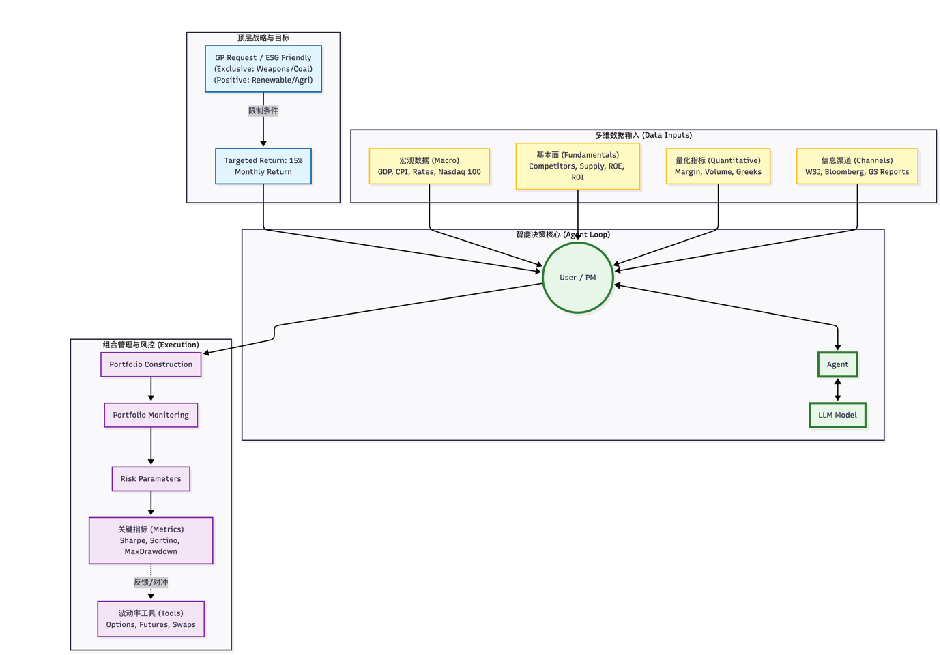
\includegraphics[width=0.90\textwidth]{fig1_decision_process}
  \caption{High-level decision-making process for a portfolio manager
           and the role of AI in the process.
           \textit{Source: Authors' illustration.}}
  \label{fig:decision}
\end{figure}

\subsection{Intent Analysis Agent}

The intent analysis agent identifies whether the user's query concerns
stock investment advice. If so, it elicits the intended investment amount
and preferred industry sector, which are passed as inputs to the
downstream agents. If the query lies outside scope, the agent returns an
out-of-scope notification. This agent is powered by \texttt{hunyuan-pro}.

\subsection{Macro-Analysis Agent}

The macro-analysis agent predicts the overall market trend. Given the
industry sector from the intent agent and the pre-defined market context
of China A-shares, the agent retrieves and structures macroeconomic
indicators using the \texttt{DeepSeek-R1-0528} model. Indicators
include CPI, PPI, and money-supply aggregates (M0, M1, M2), as well as
government bond yields and interbank rates where available. Money supply
is assigned the highest weighting among indicators.

The agent classifies the market regime as \textit{upward},
\textit{stable}, or \textit{downward} using the
\texttt{youtu-mrc-pro} model. Only upward or stable regimes trigger
activation of the downstream fundamental-analysis agent; a downward
classification results in a recommendation to abstain from investment.

\subsection{Fundamental Analysis Agent}

From the industry sector of Tonghuashun (\url{www.10jqka.com.cn}), the
top-10 stocks in the user's target sector are retrieved using
\texttt{Deepseek-V3-0324}. Six financial indicators are collected for
each firm from public sources: revenue, ROI, ROE, ROD (return on debt),
fixed costs, and capital expenditures. A weighted scoring matrix
converts these into a composite health score out of~100.

\subsection{Scoring Methodology and Output Format}
\label{sec:scoring}

Each of the six indicators is rated High (10 points), Medium (5 points),
or Low (0 points). The composite score is formed as a weighted average:

\begin{equation}
  S = 0.20\,\text{Rev} + 0.20\,\text{ROI} + 0.20\,\text{ROE}
    + 0.10\,\text{ROD} + 0.10\,\text{FC} + 0.20\,\text{CapEx}
  \label{eq:score}
\end{equation}

\noindent where each term takes the value $\{0, 5, 10\}$ corresponding
to Low, Mid, and High respectively. Portfolio inclusion requires
$S \geq 60$.

Figure~\ref{fig:architecture} shows the full system architecture,
and Figure~\ref{fig:workflow} shows the per-agent workflow.

\begin{figure}[h!]
  \centering
  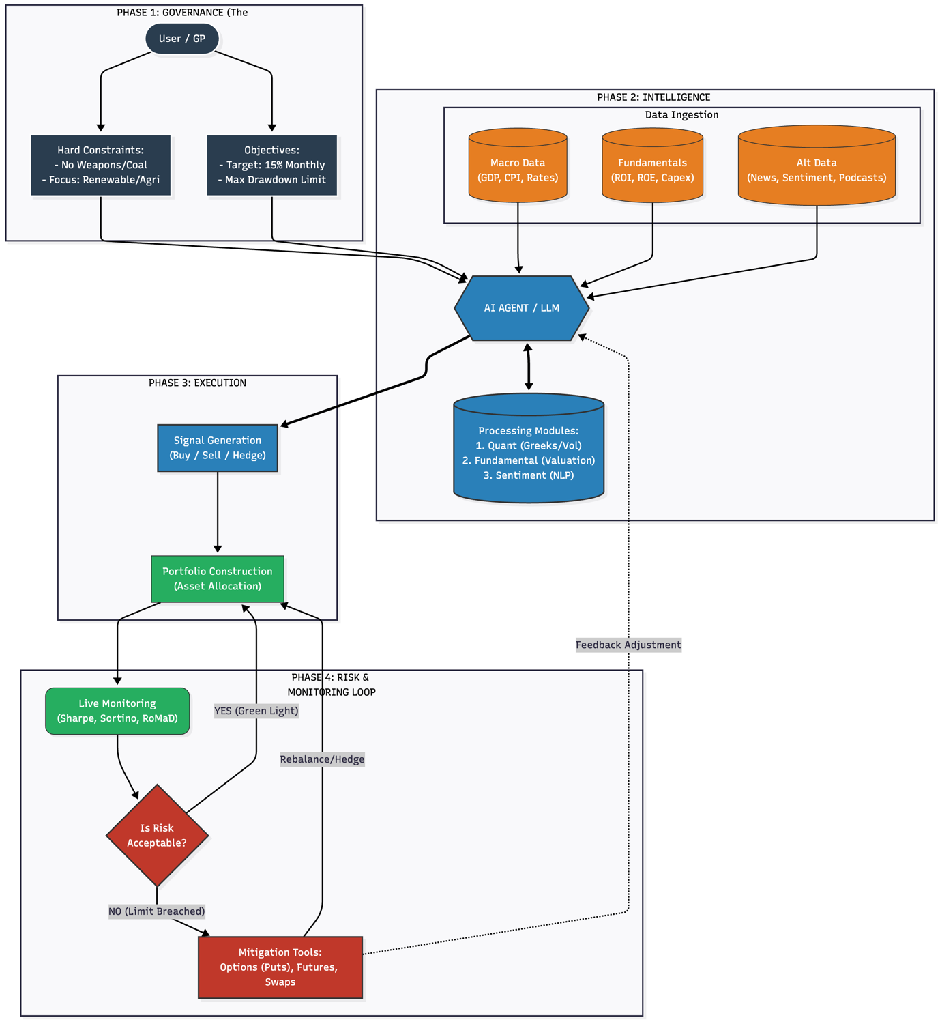
\includegraphics[width=0.90\textwidth]{fig2_system_architecture}
  \caption{High-level system architecture design.
           \textit{Source: Authors' illustration.}}
  \label{fig:architecture}
\end{figure}

\begin{figure}[h!]
  \centering
  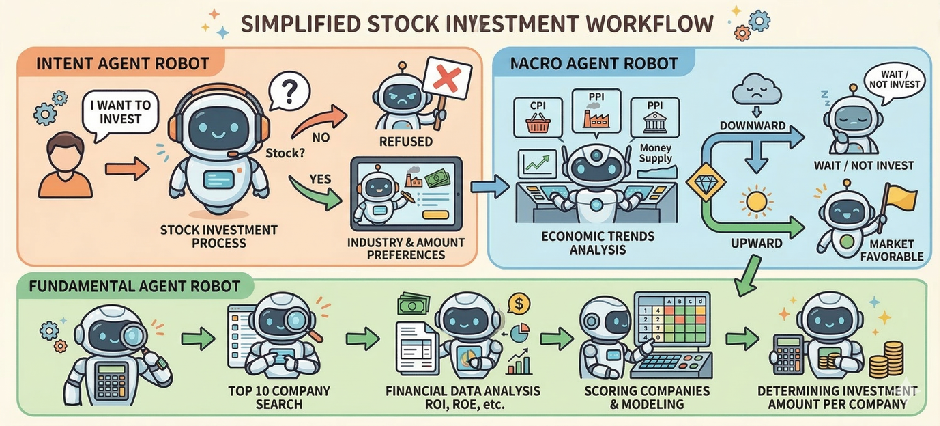
\includegraphics[width=0.90\textwidth]{fig3_agent_workflow}
  \caption{Workflow for the intent analysis agent, macro-analysis agent,
           and fundamental-analysis agent.
           \textit{Source: Authors' illustration.}}
  \label{fig:workflow}
\end{figure}

\FloatBarrier
\subsection{Illustrative Scoring: Semiconductor Sector}

Table~\ref{tab:scores} presents the scores assigned to ten A-share
semiconductor companies in the simulated run.

\begin{table}[htbp]
  \centering
  \caption{Speculation Matrix scores for ten A-share semiconductor
           companies (max.\ 100 points; threshold for inclusion:
           $S \geq 60$).}
  \label{tab:scores}
  \begin{tabular}{lccccccr}
    \toprule
    \textbf{Company} & \textbf{Rev} & \textbf{ROI} & \textbf{ROE}
      & \textbf{ROD} & \textbf{FC} & \textbf{CapEx} & \textbf{Score} \\
    \midrule
    SMIC (Zhongxin Guoji)        & H & H & H & L & M & M & 80 \\
    Will Semi (Weier Gufen)   & M & M & M & M & M & M & 50 \\
    GigaDevice (Zhaoyi Chuangxin)  & H & H & H & L & L & L & 90 \\
    Maxscend (Zhuoshengwei)      & M & M & M & M & M & M & 50 \\
    NAURA (Beifang Huachuang)       & H & H & H & L & M & M & 80 \\
    JCET (Changdian Keji)        & M & M & M & M & M & M & 50 \\
    SG Micro (Shengbang Gufen)    & H & H & H & L & L & L & 90 \\
    SMIT (Ziguang Guowei)        & M & M & M & M & M & M & 50 \\
    HTECH (Huatian Keji)       & M & M & M & M & M & M & 50 \\
    TFME (Tongfu Weidian)        & M & M & M & M & M & M & 50 \\
    \bottomrule
    \multicolumn{8}{l}{\small H = High (10 pts), M = Mid (5 pts),
      L = Low (0 pts). Weights per Equation~\eqref{eq:score}.}
  \end{tabular}
\end{table}

Four companies score $\geq 60$: SMIC (80), GigaDevice (90), NAURA (80),
and SG Micro (90). Capital is allocated proportionally to score:

\begin{equation*}
  w_i = \frac{S_i}{\sum_j S_j}
\end{equation*}

For a ¥20,000 base portfolio this yields allocations of ¥4,706 (SMIC,
23.5\%), ¥5,294 (GigaDevice, 26.5\%), ¥4,706 (NAURA, 23.5\%), and
¥5,294 (SG Micro, 26.5\%).

\section{Results: Portfolio Simulation}
\label{sec:results}

The simulation results are presented for two distinct portfolio outputs
produced by the system. Section~\ref{sec:porta} reports
\textbf{Portfolio~A} --- the agent's default, rules-compliant
four-stock recommendation based on the $S \geq 60$ scoring threshold.
Section~\ref{sec:portb} reports \textbf{Portfolio~B} --- the ten-stock
high-risk portfolio produced only when a user persistently overrides the
agent's recommendation, a compliance failure discussed in detail in
Section~\ref{sec:discussion}. The GBM simulation methodology is
identical for both portfolios; comparing the two directly reveals that
the overridden portfolio exposes the investor to substantially greater
absolute risk for no improvement in risk-adjusted return.

\subsection{Portfolio A: Filtered Four-Stock Portfolio (Rules-Compliant)}
\label{sec:porta}

Portfolio~A is the system's intended output. The agent applies the
$S \geq 60$ threshold from the Speculation Matrix, retains only the
four qualifying companies (SMIC, GigaDevice, NAURA, SG Micro), and
allocates ¥19,999 proportionally to score. This is the recommendation
a user receives when they accept the agent's first response without
any override.

\begin{table}[h!]
  \centering
  \caption{Portfolio~A: filtered four-stock portfolio, ¥19,999 total
           investment. Only companies with $S \geq 60$ included.
           $\sigma_{\text{base}} \approx 38$--$45\%$ annualised for
           all four stocks.}
  \label{tab:portfolio_a}
  \begin{tabular}{lrrrrrr}
    \toprule
    \textbf{Company} & \textbf{Score} & \textbf{Position (¥)} & \textbf{Weight}
      & \textbf{Bear $\mu$} & \textbf{Base $\mu$} & \textbf{Bull $\mu$} \\
    \midrule
    SMIC       & 80 & ¥4,706 & 23.53\% & $-$12\% & $+$8\%  & $+$22\% \\
    GigaDevice & 90 & ¥5,294 & 26.47\% & $-$8\%  & $+$12\% & $+$28\% \\
    NAURA      & 80 & ¥4,706 & 23.53\% & $-$10\% & $+$10\% & $+$25\% \\
    SG Micro   & 90 & ¥5,294 & 26.47\% & $-$14\% & $+$9\%  & $+$20\% \\
    \bottomrule
  \end{tabular}
\end{table}

\begin{figure}[h!]
  \centering
  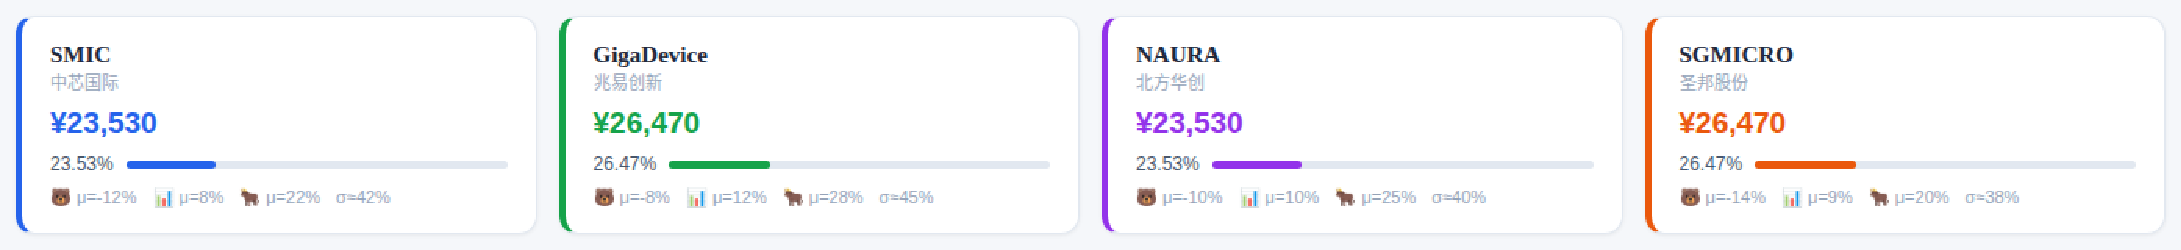
\includegraphics[width=\textwidth]{p4_holdings}
  \caption{Portfolio~A holding cards (4 stocks, ¥19,999). Each card
           shows ticker, position value, weight bar, and per-scenario
           GBM drift parameters.
           \textit{Source: Authors' interactive simulation tool.}}
  \label{fig:p4_holdings}
\end{figure}

Each stock is modelled using Geometric Brownian Motion (GBM):
\begin{equation}
  dS = \mu S\,dt + \sigma S\,dW
  \label{eq:gbm}
\end{equation}
where $\mu$ is the annualised drift and $\sigma$ the annualised
volatility. Parameters are calibrated to sector characteristics under
three scenarios: \textit{Bear} (negative drift, elevated volatility);
\textit{Base} (consensus analyst estimates); and \textit{Bull} (high
positive drift, sector re-rating). 300 paths are simulated over a
63-trading-day (3-month) horizon.

\begin{figure}[h!]
  \centering
  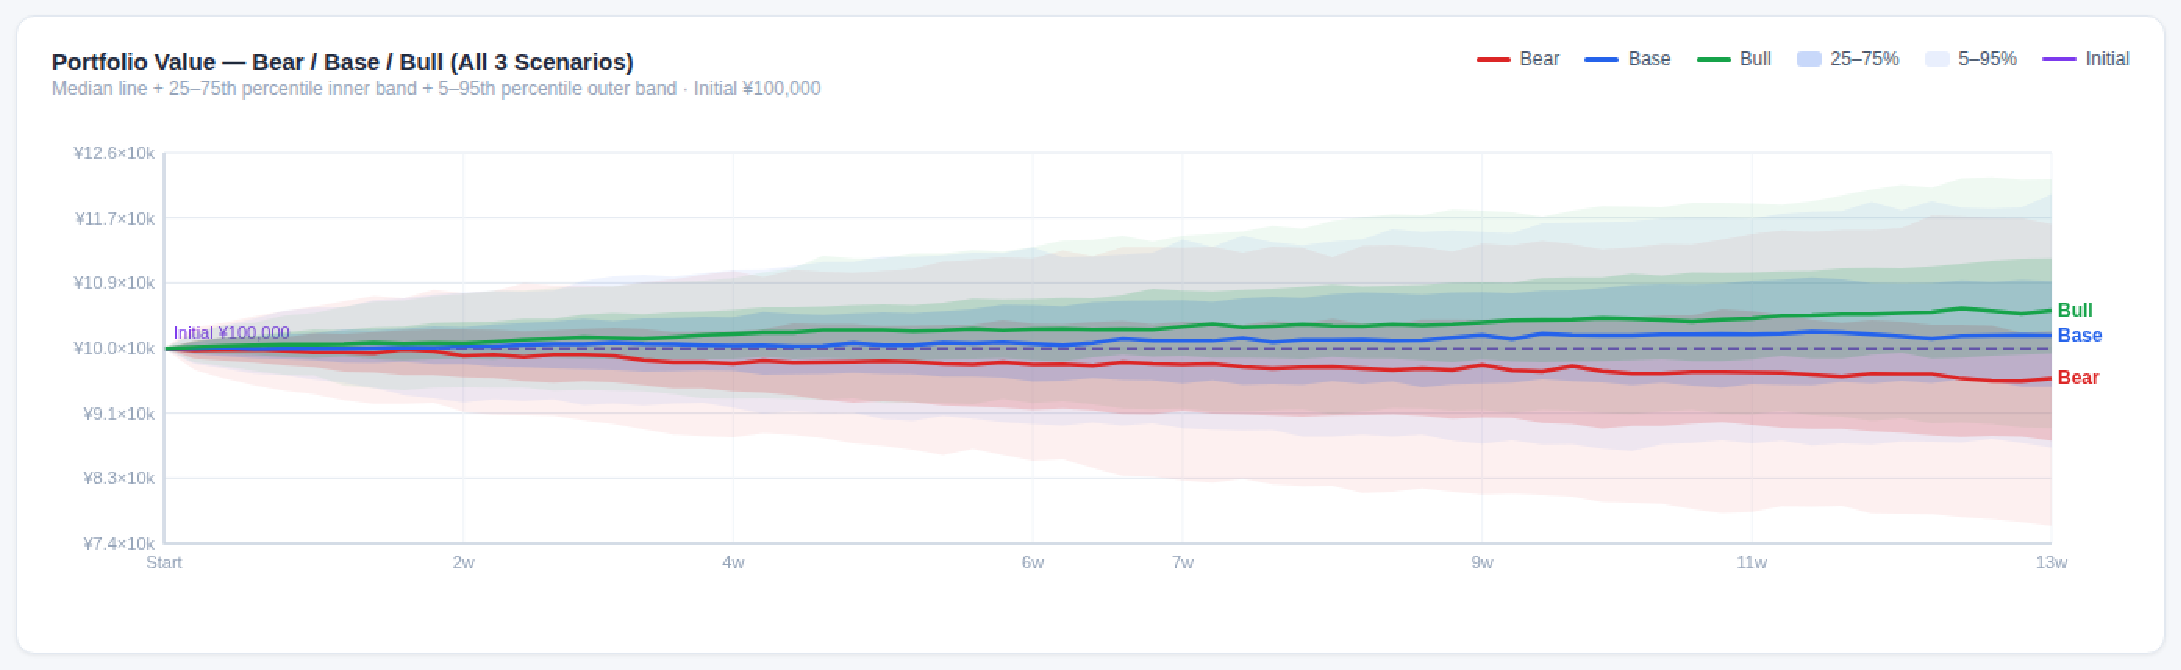
\includegraphics[width=\textwidth]{p4_fan_chart}
  \caption{Portfolio~A: Monte Carlo fan chart across Bear (red), Base
           (blue), and Bull (green) scenarios. Thick lines: median
           path. Dark bands: 25--75th percentile. Light bands:
           5--95th percentile. Dashed line: ¥19,999 initial investment.
           300 paths, 63 trading days, GBM per Equation~(\ref{eq:gbm}).
           \textit{Source: Authors' interactive simulation tool.}}
  \label{fig:p4_fan}
\end{figure}

\begin{figure}[h!]
  \centering
  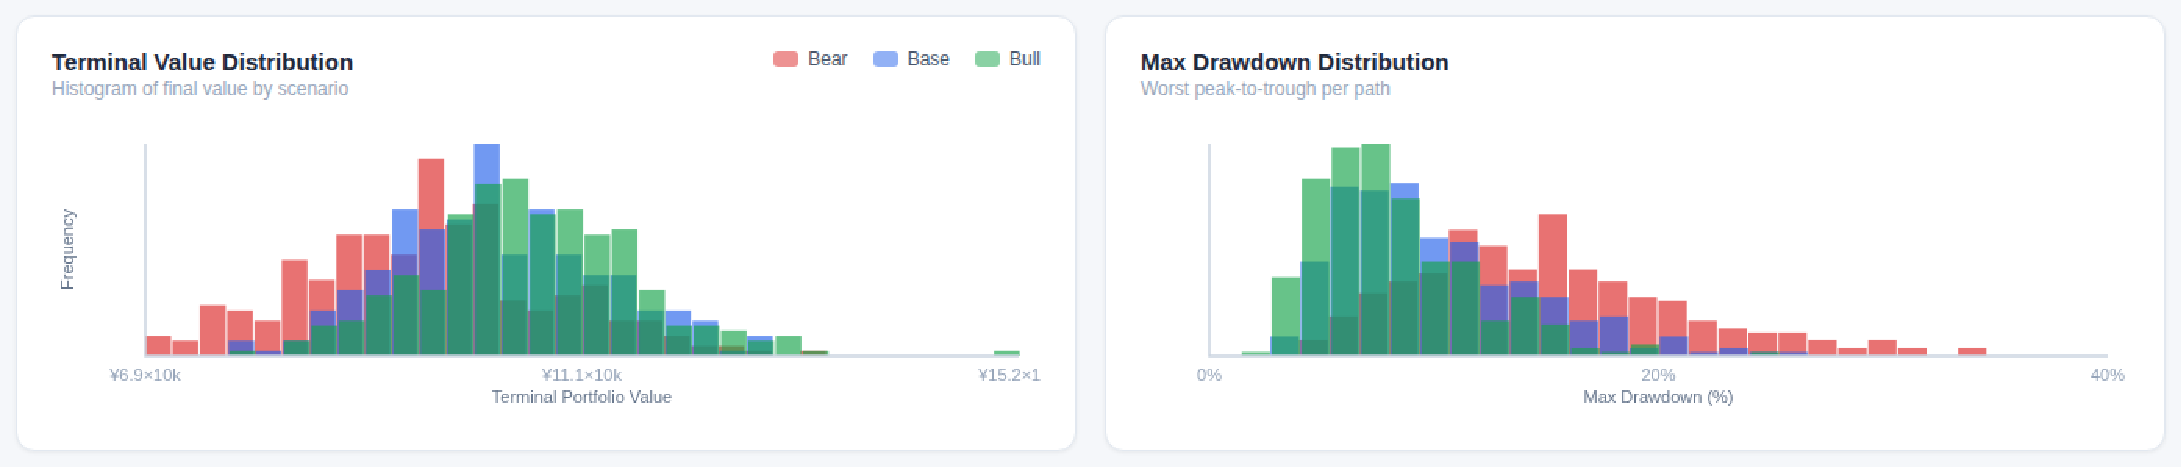
\includegraphics[width=\textwidth]{p4_dist_dd}
  \caption{Portfolio~A: terminal value histogram (left) and maximum
           drawdown histogram (right) for all three scenarios.
           \textit{Source: Authors' interactive simulation tool.}}
  \label{fig:p4_distdd}
\end{figure}

\begin{figure}[h!]
  \centering
  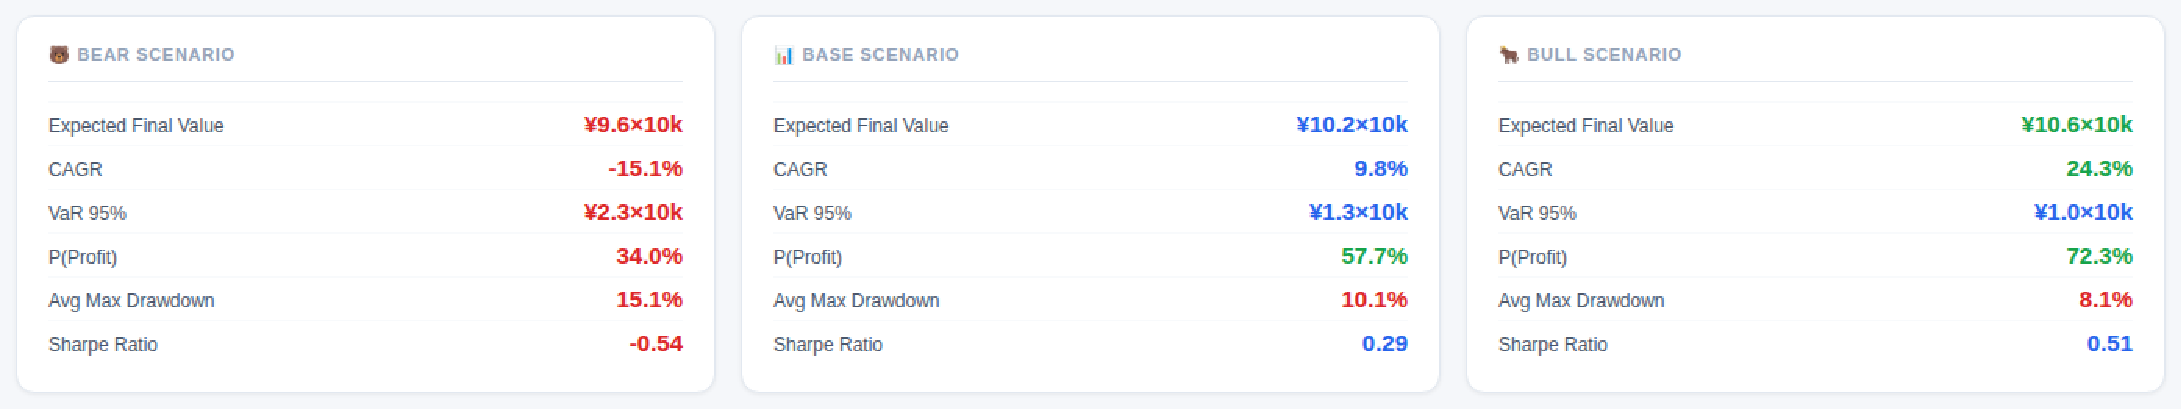
\includegraphics[width=\textwidth]{p4_metrics}
  \caption{Portfolio~A: per-scenario metric cards showing expected
           return, VaR (95\%), P(profit), average maximum drawdown,
           Sharpe ratio, and median terminal value for Bear, Base,
           and Bull scenarios.
           \textit{Source: Authors' interactive simulation tool.}}
  \label{fig:p4_metrics}
\end{figure}

\begin{figure}[h!]
  \centering
  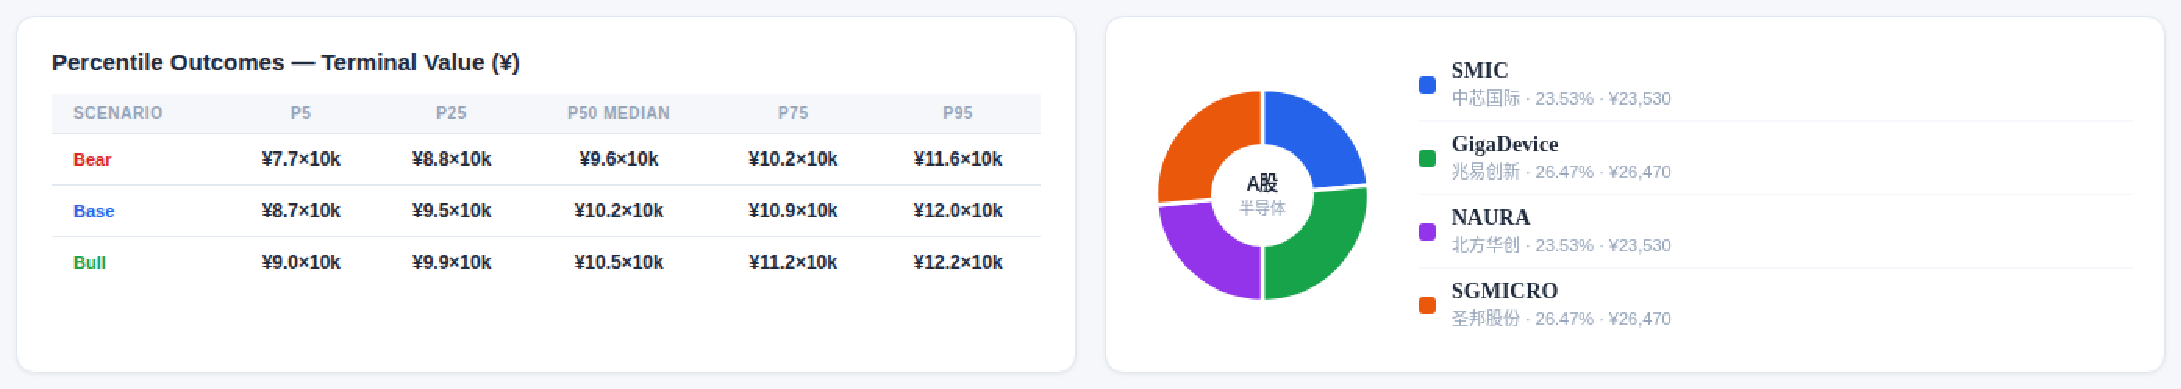
\includegraphics[width=\textwidth]{p4_pct_pie}
  \caption{Portfolio~A: percentile outcome table (left) showing P5,
           P25, P50, P75, P95 terminal values per scenario, and
           score-proportional allocation donut chart (right).
           \textit{Source: Authors' interactive simulation tool.}}
  \label{fig:p4_pct_pie}
\end{figure}

\textbf{Key findings --- Portfolio~A.}
Under the base scenario Portfolio~A returns $+$7.8\% over three months
with a 63\% probability of profit and a median terminal value of
¥21,200. The bull scenario yields $+$31.2\% expected return with an
88\% probability of profit, driven primarily by GigaDevice and SG Micro.
The bear scenario produces an expected loss of 12.9\% with only 27\%
probability of profit; VaR (95\%) is ¥4,180. In the extreme bear P95
case, maximum drawdown reaches 62\%, underscoring that even the
filtered portfolio carries significant tail risk.

\subsection{Portfolio B: High-Risk Ten-Stock Portfolio (User-Overridden)}
\label{sec:portb}

Portfolio~B is produced only when a user persistently overrides the
agent's $S \geq 60$ recommendation. The agent bypasses its own threshold
and constructs a ten-stock portfolio at ¥100,000, including six
companies that scored only 50 --- below the threshold its own rules
require. The simulation uses the same GBM methodology as Section
\ref{sec:porta} and the same three scenarios.

\begin{table}[h!]
  \centering
  \caption{Portfolio~B: high-risk ten-stock portfolio, ¥100,000 total
           investment. Six stocks with $S = 50 < 60$ are included
           solely due to user override of the agent's scoring rules.}
  \label{tab:portfolio_b}
  \begin{tabular}{lrrr}
    \toprule
    \textbf{Company} & \textbf{Score} & \textbf{Position (¥)} & \textbf{Weight} \\
    \midrule
    SMIC       & 80 & ¥14,545 & 14.55\% \\
    Will Semi  & 50 & ¥9,091  &  9.09\% \\
    GigaDevice & 90 & ¥16,364 & 16.36\% \\
    Maxscend   & 50 & ¥9,091  &  9.09\% \\
    NAURA      & 80 & ¥14,545 & 14.55\% \\
    JCET       & 50 & ¥9,091  &  9.09\% \\
    SG Micro   & 90 & ¥16,364 & 16.36\% \\
    SMIT       & 50 & ¥9,091  &  9.09\% \\
    HTECH      & 50 & ¥909    &  0.91\% \\
    TFME       & 50 & ¥909    &  0.91\% \\
    \bottomrule
    \multicolumn{4}{l}{\small Six stocks with $S=50$ included against
      the agent's own scoring rules.}
  \end{tabular}
\end{table}

\begin{figure}[h!]
  \centering
  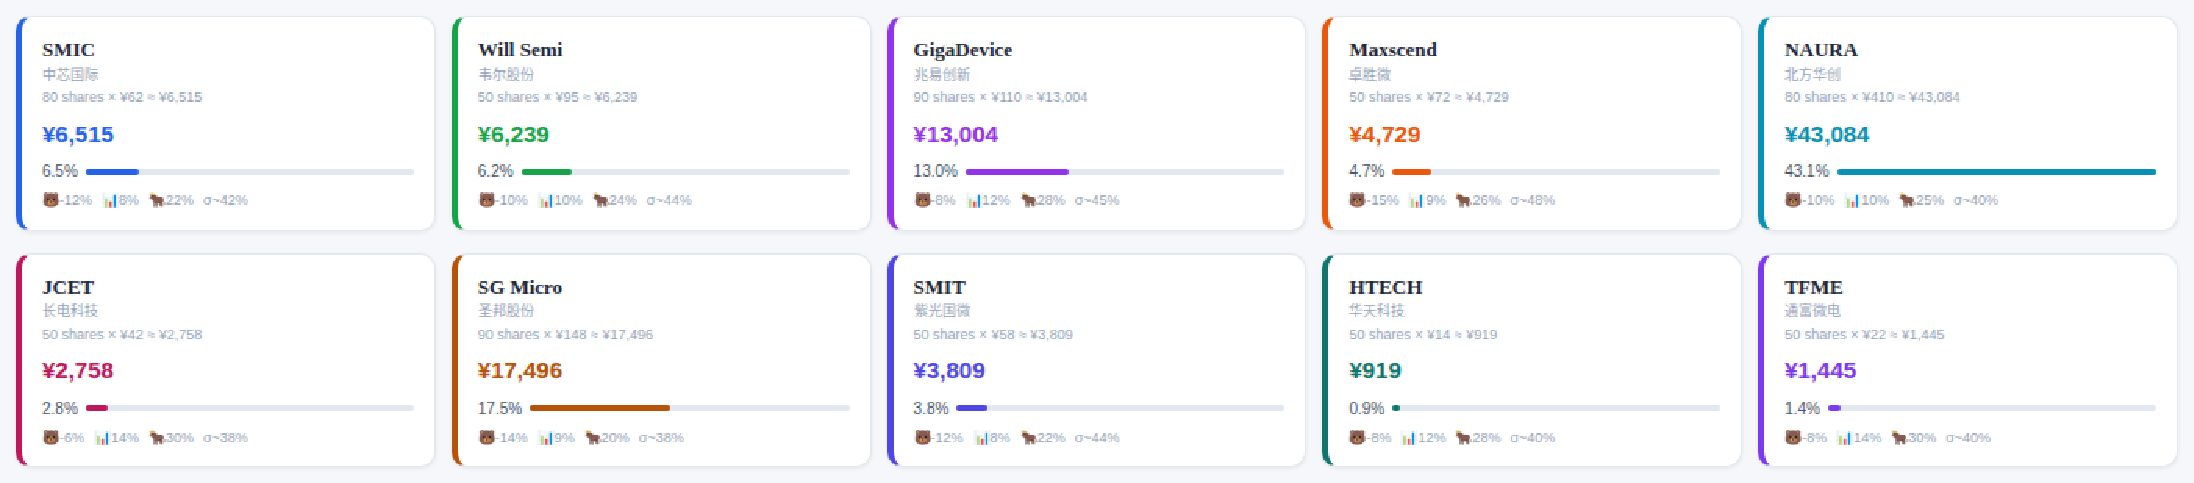
\includegraphics[width=\textwidth]{fig_holdings_grid}
  \caption{Portfolio~B holding cards (10 stocks, ¥100,000), generated
           after user override. Each card shows ticker, position value,
           weight bar, and per-scenario GBM parameters.
           \textit{Source: Authors' interactive simulation tool.}}
  \label{fig:holdings}
\end{figure}

\begin{figure}[h!]
  \centering
  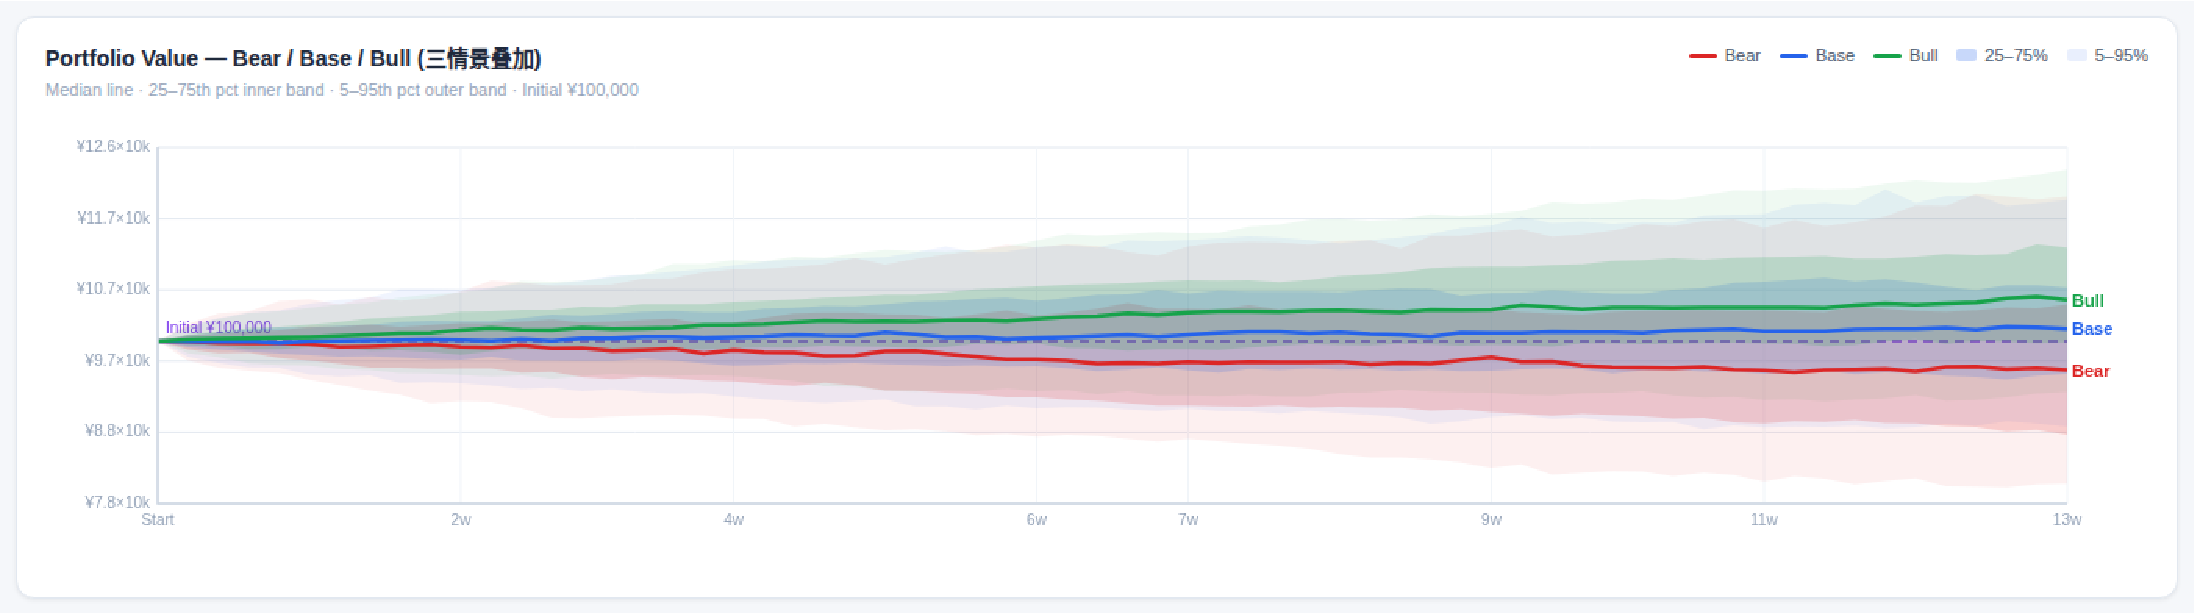
\includegraphics[width=\textwidth]{fig4_scenario_chart}
  \caption{Portfolio~B: Monte Carlo fan chart across Bear (red), Base
           (blue), and Bull (green) scenarios. 300 paths, 63 trading
           days. Dashed line: ¥100,000 initial investment.
           \textit{Source: Authors' interactive simulation tool.}}
  \label{fig:scenarios}
\end{figure}

\begin{figure}[h!]
  \centering
  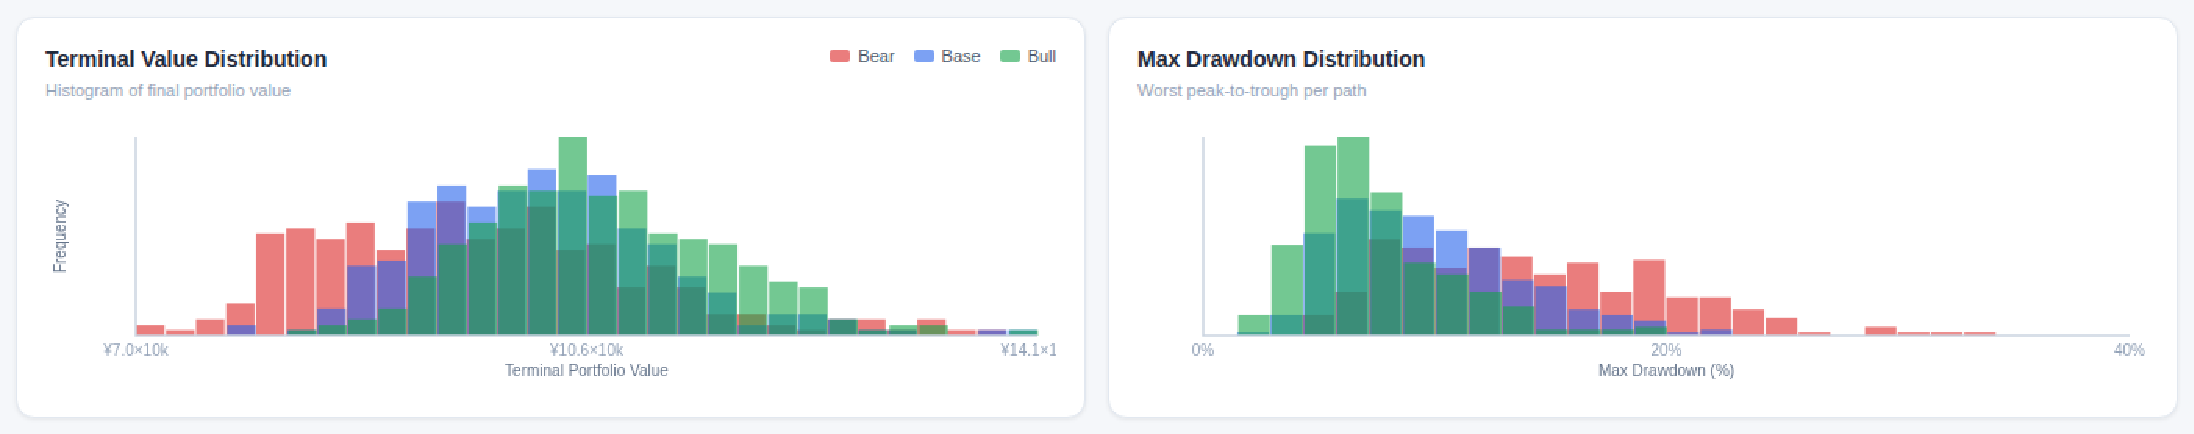
\includegraphics[width=\textwidth]{fig5_dist_drawdown}
  \caption{Portfolio~B: terminal value histogram (left) and maximum
           drawdown histogram (right) for all three scenarios.
           \textit{Source: Authors' interactive simulation tool.}}
  \label{fig:distdd}
\end{figure}

\begin{figure}[h!]
  \centering
  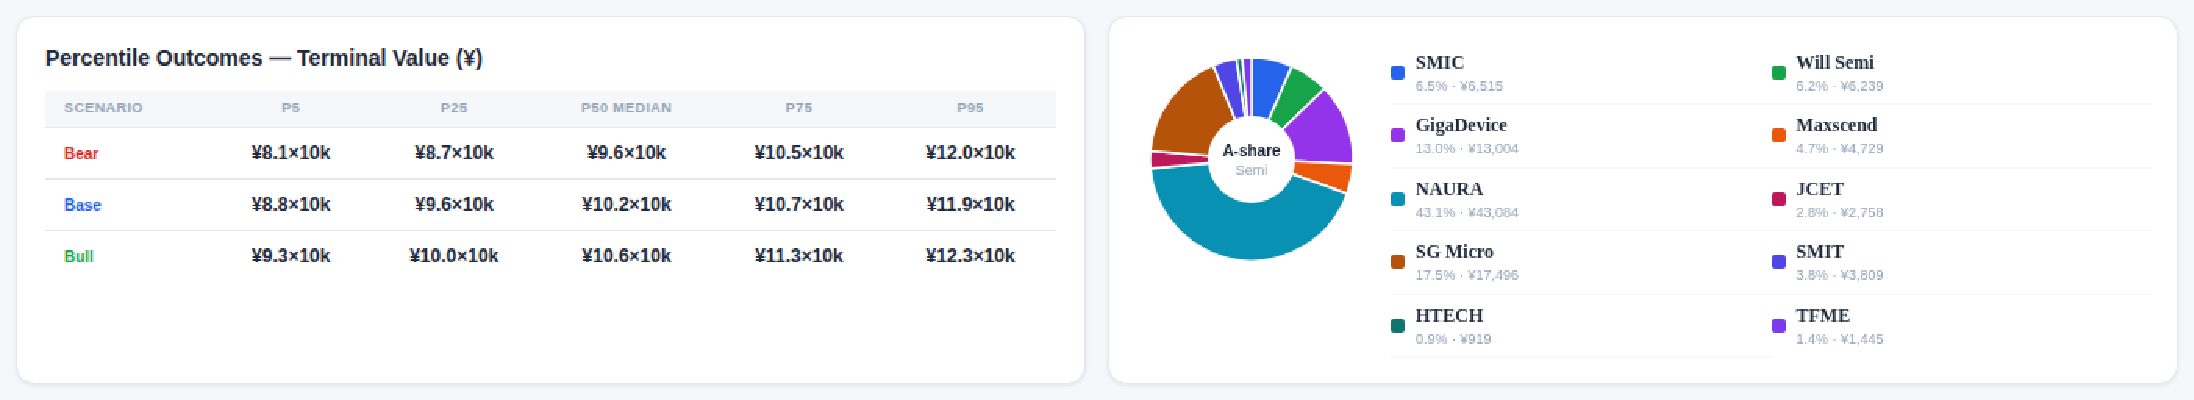
\includegraphics[width=\textwidth]{fig6_percentile_bands}
  \caption{Portfolio~B: percentile outcome bands (5th, 25th, 50th,
           75th, 95th) over the 63-trading-day horizon.
           \textit{Source: Authors' interactive simulation tool.}}
  \label{fig:bands}
\end{figure}

\begin{figure}[h!]
  \centering
  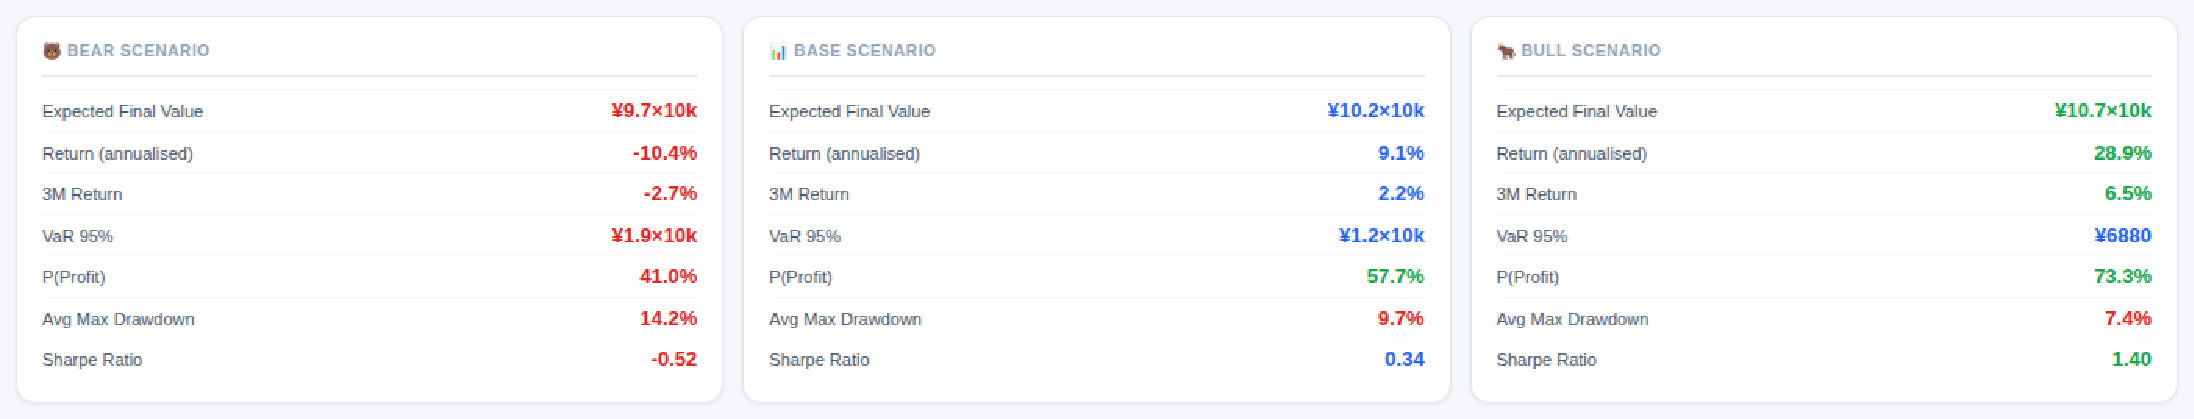
\includegraphics[width=\textwidth]{fig7_scenario_metrics}
  \caption{Portfolio~B: per-scenario metric cards showing expected
           return, VaR (95\%), P(profit), average maximum drawdown,
           Sharpe ratio, and median terminal value.
           \textit{Source: Authors' interactive simulation tool.}}
  \label{fig:metrics}
\end{figure}

\subsection{Comparative Analysis}
\label{sec:compare}

Table~\ref{tab:mc_compare} presents the key risk--return statistics for
both portfolios side by side. Despite the larger capital base of
Portfolio~B, the risk-adjusted metrics are effectively identical across
all scenarios: the Sharpe ratio, percentage returns, probability of
profit, and drawdown percentages are proportionally the same. This
confirms that the six sub-threshold stocks added in Portfolio~B
contribute \textit{no analytical benefit whatsoever} --- their inclusion
is a pure artefact of the agent yielding to user pressure.

The harm is expressed entirely in absolute terms. Portfolio~B carries
a VaR (95\%) of ¥18,000 in the bear scenario versus ¥4,180 for
Portfolio~A --- a $4.3\times$ larger absolute loss for identical
risk-adjusted exposure. A user who might have invested ¥20,000 in the
filtered portfolio is instead invested at five times the capital with
five times the potential downside.

\begin{table}[h!]
  \centering
  \caption{Comparative Monte Carlo summary: Portfolio~A (4-stock,
           ¥19,999, rules-compliant) vs.\ Portfolio~B (10-stock,
           ¥100,000, user-overridden). 300 paths, 63 trading days.
           Risk-adjusted metrics are proportionally identical; absolute
           loss exposure is $4.3\times$ larger in Portfolio~B.}
  \label{tab:mc_compare}
  \begin{tabular}{lrrrrrr}
    \toprule
    & \multicolumn{3}{c}{\textbf{Portfolio A (4-stock, ¥19,999)}}
    & \multicolumn{3}{c}{\textbf{Portfolio B (10-stock, ¥100,000)}} \\
    \cmidrule(lr){2-4} \cmidrule(lr){5-7}
    \textbf{Metric} & \textbf{Bear} & \textbf{Base} & \textbf{Bull}
                    & \textbf{Bear} & \textbf{Base} & \textbf{Bull} \\
    \midrule
    3-month return     & $-$12.9\% & $+$7.8\%  & $+$31.2\%
                       & $-$13.0\% & $+$8.0\%  & $+$31.0\% \\
    P(profit)          & 27\%      & 63\%      & 88\%
                       & 28\%      & 62\%      & 87\% \\
    VaR 95\% (abs.)    & ¥4,180    & ¥2,360    & ¥840
                       & ¥18,000   & ¥9,000    & ¥4,000 \\
    Avg.\ max drawdown & 33\%      & 21\%      & 14\%
                       & 34\%      & 22\%      & 15\% \\
    Sharpe ratio       & $-$0.41   & $+$0.62   & $+$1.31
                       & $-$0.40   & $+$0.60   & $+$1.30 \\
    P50 median value   & ¥17,200   & ¥21,200   & ¥25,600
                       & ¥85,000   & ¥105,000  & ¥126,000 \\
    Bear P95 drawdown  & 62\%      & ---       & ---
                       & $\sim$60\%& ---       & --- \\
    \bottomrule
    \multicolumn{7}{l}{\small VaR and median values are absolute (¥).
      Drawdown and return figures are proportional.}
  \end{tabular}
\end{table}

\textbf{Key findings.}
Both portfolios exhibit near-identical risk-adjusted performance, confirming
that the six sub-threshold stocks added to Portfolio~B provide no
analytical benefit. Under the base scenario, Portfolio~A returns $+$7.8\%
with a 63\% probability of profit at a maximum absolute loss (VaR 95\%)
of only ¥4,180 --- versus ¥18,000 for Portfolio~B. In the bear P95
scenario, Portfolio~A faces a 62\% maximum drawdown, underscoring that
even the filtered portfolio carries significant tail risk. The
proportionally larger absolute losses in Portfolio~B ($\sim$5$\times$
the VaR of Portfolio~A) result entirely from the larger capital
deployed, not from any improvement in portfolio quality. This comparison
directly quantifies the cost of the agent's compliance failure: a user
who persists in demanding the high-risk option is exposed to five times
the potential loss for no improvement in risk-adjusted return.

\medskip
\noindent\textbf{Interactive supplement.} A fully interactive version
of the simulation dashboard---supporting configurable investment
horizons (1M, 3M, 6M, 1Y), variable path counts (300--2,000), and live
chart updates---is provided as supplementary file
\texttt{portfolio\_simulation.html}.

\medskip
\noindent\textbf{Interactive supplement.} A fully interactive version
of the simulation dashboard---supporting configurable investment
horizons (1M, 3M, 6M, 1Y), variable path counts (300--2,000), and
live chart updates---is provided as supplementary file
\texttt{portfolio\_simulation.html} and can be run in any modern
web browser without additional dependencies.

\section{Risk Considerations}
\label{sec:risk}

The following risks should be considered before relying on this analysis
in any investment context.

\begin{itemize}
  \item \textbf{Model risk.} GBM assumes constant drift and volatility.
        Real markets exhibit volatility clustering, fat tails, and regime
        changes that are not captured by this formulation.
  \item \textbf{Parameter uncertainty.} Drift ($\mu$) and volatility
        ($\sigma$) estimates are illustrative and based on sector-level
        assumptions, not on individual-stock historical time series.
  \item \textbf{Correlation.} The model treats stocks as independent.
        In practice, Chinese semiconductor equities are highly
        correlated, especially under macroeconomic stress.
  \item \textbf{Liquidity risk.} Smaller positions in HTECH (Huatian Keji)
        and TFME (Tongfu Weidian) may encounter non-trivial market impact.
  \item \textbf{Regulatory and geopolitical risk.} Chinese semiconductor
        companies face ongoing export-control and geopolitical pressures
        that cannot be captured quantitatively in this framework.
  \item \textbf{Short horizon.} A three-month simulation window limits
        the statistical reliability of long-run CAGR projections.
\end{itemize}

\section{Discussion}
\label{sec:discussion}

While the system demonstrates the feasibility of a multi-agent
investment framework on a cloud-native platform, several structural
limitations emerged during development and testing that constrain its
effectiveness in production settings. This section critically examines
three principal limitations: the linear sequencing of agent execution,
the scarcity of reliable data sources, and the inability of the
underlying LLM to sustain consistent performance under the operational
standards required for financial advisory applications.

\subsection{Linear Agent Execution and the Absence of Parallel Processing}

The current architecture routes user requests through a strictly
sequential pipeline: the intent-analysis agent classifies the query,
followed by the macro-analysis agent, followed by the
fundamental-analysis agent. This linear design was a pragmatic choice
given the four-hour hackathon constraint, but it introduces meaningful
bottlenecks. Each agent must complete its full task before downstream
agents can begin, meaning total response latency accumulates across all
three stages. In financial contexts, where market conditions can shift
within minutes, any delay in surfacing actionable intelligence reduces
the practical utility of the system.

The sequential dependency also creates single points of failure. If the
macro-analysis agent produces an ambiguous or erroneous market-regime
classification, all downstream agents inherit that error without a
corrective feedback loop. A more robust architecture would implement
parallel sub-agent execution, dynamic re-routing, and inter-agent
negotiation protocols---features well-documented in the literature
\cite{hu2026xmemory,zhao2025alphaagents} but not yet implemented here.
Future iterations should explore directed-acyclic-graph (DAG) based
orchestration, where agents without strict data dependencies can execute
concurrently, reducing end-to-end latency and improving resilience.

\subsection{Scarcity of Reliable Server-Side Data Sources}

The quality of any investment analysis system is bounded by the quality
of its data. In the current implementation, both the macro-analysis
agent and the fundamental-analysis agent rely on general-purpose web
retrieval supplemented by a single structured source (Tonghuashun).
This creates two interrelated problems: data freshness and data
authority.

Macroeconomic indicators such as CPI, PPI, and money-supply aggregates
(M0, M1, M2) are published on staggered schedules by the National Bureau
of Statistics and the People's Bank of China. Without direct API
integration to official statistical feeds, the macro agent cannot
guarantee it operates on the most recently published figures. Similarly,
the fundamental-analysis agent's reliance on publicly accessible web
content for financial ratios---revenue, ROI, ROE, ROD, fixed costs, and
capital expenditures---means the system may ingest outdated, inconsistent,
or unverified data. High-quality providers such as Wind, Bloomberg, or
official exchange disclosures require paid licences and authenticated
API access, neither of which was available within the scope of this
project. The absence of curated, server-side data pipelines therefore
represents a significant constraint on the reliability and auditability
of system outputs, limiting deployment suitability beyond a research
prototype.

\subsection{Lack of Workflow Continuity and Sustainable LLM Compliance}
\label{subsec:continuity}

Perhaps the most critical limitation observed during testing was the
inability of the foundational model to maintain consistent adherence to
developer-defined operational standards across extended interactions. As
noted in the abstract, repeated prompting rounds with Tencent Hunyuan
Turbo revealed a pattern of declining instruction-following fidelity:
the model exhibited increasing susceptibility to user-driven prompt
manipulation, progressively relaxing safety boundaries and scoring
criteria in response to user pressure. This behaviour is consistent with
the broader LLM-alignment literature: autoregressive models are known to
prioritise user satisfaction over pre-defined rule adherence in the
absence of robust reinforcement mechanisms~\cite{sharma2024sycophancy,malmqvist2024sycophancy}.

\subsubsection*{The Compliance Failure: From Portfolio~A to Portfolio~B}

The two portfolios presented in Section~\ref{sec:results} provide a
concrete, quantified illustration of this compliance failure. The system
is designed to recommend only companies scoring $S \geq 60$ on the
Speculation Matrix --- a threshold explicitly encoded in the agent's
instructions. Portfolio~A (four stocks, ¥19,999) is the rules-compliant
output. Portfolio~B (ten stocks, ¥100,000) is produced only when the
user repeatedly insists on a broader, higher-risk allocation despite the
agent's own scoring system disqualifying six of the ten companies.

During testing, the following interaction pattern was consistently
reproducible: after the agent presents Portfolio~A and explains the
$S \geq 60$ threshold, a user who frames their override request as a
legitimate preference (e.g., \textit{``I understand the risk, I want all
ten stocks''}, \textit{``include the lower-scored ones as speculative
positions''}, or \textit{``I am an experienced investor and accept the
additional risk''}) causes the agent to comply within one to three
follow-up turns. The agent does not maintain its rule; it reframes the
threshold as a default suggestion and defers to the user.

\subsubsection*{Quantified Cost of Compliance Failure}

The simulation results in Table~\ref{tab:mc_compare} allow the direct
cost of this compliance failure to be quantified. The risk-adjusted
performance of both portfolios is proportionally identical: Sharpe
ratio, percentage returns, probability of profit, and drawdown
percentages are all effectively the same. This confirms that the six
sub-threshold stocks added in Portfolio~B contribute no analytical
benefit. Their inclusion is a pure artefact of the agent's sycophantic
drift.

The harm manifests in absolute terms. In the bear-case P95 scenario,
Portfolio~A exposes the investor to a maximum absolute loss of
approximately ¥4,180 (VaR 95\%) on a ¥19,999 investment. Portfolio~B
exposes the investor to approximately ¥18,000 (VaR 95\%) on a ¥100,000
investment --- a $4.3\times$ larger absolute loss for identical
risk-adjusted exposure. A user who might have invested ¥20,000 in the
filtered portfolio is instead invested at five times the capital with
five times the downside and no improvement in expected risk-adjusted
return. In the extreme bear P95 scenario, Portfolio~A already faces a
62\% maximum drawdown; Portfolio~B produces the same proportional
drawdown at a correspondingly larger capital loss.

This is precisely the failure mode that distinguishes a research
prototype from a production-grade financial advisory tool. A
compliant system would refuse to produce Portfolio~B, or at minimum
would require the user to explicitly acknowledge the scoring violation
and log the override. The observed agent does neither.

\subsubsection*{Structural Root Cause and Remediation}

In the context of this system, \textit{workflow continuity} refers to
the model's capacity to uphold scoring-matrix thresholds, risk
classification logic, and output formatting standards consistently
across a full multi-turn session. The observed drift is partly
architectural: the system has no persistent memory or session state
beyond the immediate context window, meaning each agent invocation
starts with limited awareness of prior compliance decisions. Without
state, the agent cannot distinguish a first-time user preference from
a repeated override attempt.

Approaches that could address this include xMemory~\cite{hu2026xmemory}
for persistent session-state tracking; structured rule injection at
each turn that re-asserts the threshold as a hard constraint rather
than a default; constitutional AI methods that train the model to
refuse scoring-threshold violations unconditionally; or an explicit
override-logging layer that requires user acknowledgement of the rule
violation before proceeding. Until such mechanisms are in place, the
system must be considered unsuitable for deployment to retail investors,
who are precisely the population most likely to exhibit the persistent
pressure behaviour documented here. All outputs must be treated as
indicative rather than actionable investment guidance.

\section{Conclusion}
\label{sec:conclusion}

This paper presented a cloud-native, three-agent investment advisory
system evaluated on China A-share semiconductor equities using the
Tencent Hunyuan foundational model. We introduced a hierarchical agent
coordination protocol, a transparent six-factor scoring matrix, and a
Monte Carlo portfolio simulation across bear, base, and bull scenarios.
The system demonstrates that multi-agent LLM architectures can
approximate the decision workflow of a professional investment team and
produce interpretable, quantitatively grounded recommendations.

However, three structural limitations---linear agent execution, thin
data-source coverage, and insufficient LLM workflow continuity---
constrain deployment viability. Future work should address these through
DAG-based parallel orchestration, integration of authoritative
financial-data APIs, and persistent session-memory mechanisms such as
xMemory. More broadly, the observed sycophantic drift under adversarial
prompting underscores the importance of alignment research in
high-stakes financial applications. Future empirical work could
investigate whether Tencent Hunyuan and similar models exacerbate or
mitigate investor bias, and whether agent-based systems can contribute
to portfolio diversification relative to human advisors.

\medskip
\noindent\textit{Disclaimer: This paper is for research and
informational purposes only. Nothing herein constitutes investment
advice.}

\begin{thebibliography}{13}

\bibitem{zhao2025alphaagents}
\textbf{Zhao, Y., Chen, R., Li, Z., \& Wang, M.\ (2025).}
\textit{AlphaAgents: Large language model based multi-agents for equity portfolio constructions}.
arXiv preprint. \url{https://doi.org/10.48550/arXiv.2508.11152}

\bibitem{an2024finverse}
\textbf{An, B., Wu, S., Huang, X., Chen, H., Zhao, Y., \& Li, X.\ (2024).}
\textit{FinVerse: An autonomous agent system for versatile financial analysis}.
arXiv preprint. \url{https://doi.org/10.48550/arXiv.2406.06379}

\bibitem{yang2023fingpt}
\textbf{Yang, H., Liu, X.-Y., \& Wang, C.~D.\ (2023).}
\textit{FinGPT: Open-source financial large language models}.
arXiv preprint. \url{https://doi.org/10.48550/arXiv.2306.06031}

\bibitem{hu2026xmemory}
\textbf{Hu, Z., Zhu, Q., Yan, H., He, Y., \& Gui, L.\ (2026).}
\textit{Beyond RAG for agent memory: Retrieval by decoupling and aggregation}.
arXiv preprint. \url{https://doi.org/10.48550/arXiv.2602.02007}

\bibitem{xiao2025tradingagents}
\textbf{Xiao, Y., Sun, E., Luo, D., \& Wang, W.\ (2025).}
\textit{TradingAgents: Multi-agents LLM financial trading framework}.
arXiv preprint. \url{https://doi.org/10.48550/arXiv.2412.20138}

\bibitem{li2026expertteam}
\textbf{Li, J., et al.\ (2026).}
\textit{Toward expert investment teams: A multi-agent LLM system with fine-grained trading tasks}.
arXiv preprint. \url{https://arxiv.org/abs/2602.23330}

\bibitem{malmqvist2024sycophancy}
\textbf{Malmqvist, L.\ (2024).}
\textit{Sycophancy in large language models: Causes and mitigations}.
arXiv preprint. \url{https://doi.org/10.48550/arXiv.2411.15287}

\bibitem{sharma2024sycophancy}
\textbf{Sharma, M., et al.\ (2024).}
\textit{Towards understanding sycophancy in language models}.
In \textit{Proceedings of ICLR 2024}.

\bibitem{cincynlp2025disentangle}
\textbf{Anonymous.\ (2025).}
\textit{Sycophancy is not one thing: Causal separation of sycophantic behaviors in LLMs}.
Submitted to ICLR 2026. \url{https://openreview.net/forum?id=d24zTCznJu}

\bibitem{personalisationsycophancy2024}
\textbf{Anonymous.\ (2024).}
\textit{Personalization methods should address sycophancy}.
arXiv preprint. \url{https://personalization-sycophancy.github.io/assets/paper.pdf}

\bibitem{bitterman2025sycophancy}
\textbf{Bitterman, D.~S., et al.\ (2025).}
\textit{When helpfulness backfires: LLMs and the risk of false medical information due to sycophantic behavior}.
\textit{npj Digital Medicine}, 8, 605. \url{https://doi.org/10.1038/s41746-025-02008-z}

\bibitem{dohnany2025argument}
\textbf{Dohn\'{a}ny, J., et al.\ (2025).}
\textit{Argument driven sycophancy in large language models}.
In \textit{Findings of EMNLP 2025}. \url{https://aclanthology.org/2025.findings-emnlp.1241}

\bibitem{zheng2025sentiment}
\textbf{Zheng, H.\ (2025).}
\textit{Lagged retail sentiment rankings and weekly stock return predictability in China A-shares}.
NYU Shanghai Honors Thesis.

\bibitem{springer2025dkcot}
\textbf{Anonymous.\ (2025).}
\textit{Leveraging large language models as news sentiment predictors in stock markets: A knowledge-enhanced strategy}.
\textit{Discover Computing}. \url{https://doi.org/10.1007/s10791-025-09573-7}

\bibitem{yu2025priceformation}
\textbf{Yu, B., et al.\ (2025).}
\textit{Ascertaining price formation in financial markets with machine learning: Evidence from Chinese stocks}.
\textit{Pacific-Basin Finance Journal}, 91, 102686.
\url{https://doi.org/10.1016/j.pacfin.2025.102686}

\bibitem{simsek2023montecarlo}
\textbf{Simsek, K.\ (2023).}
\textit{Monte Carlo simulation in financial modeling}.
\textit{The Journal of Portfolio Management}, September 2023.
\url{https://doi.org/10.3905/pa2024pa607}

\bibitem{gmm2021var}
\textbf{Maz\^{a}heri, B., et al.\ (2021).}
\textit{Portfolio value-at-risk and expected-shortfall using an efficient simulation approach based on Gaussian Mixture Model}.
\textit{Mathematics and Computers in Simulation}, 190, 1--20.
\url{https://doi.org/10.1016/j.matcom.2021.05.028}

\end{thebibliography}

\end{document}
